\documentclass[10pt]{article}
\usepackage[margin=0.85in,top=0.7in,bottom=0.7in]{geometry}
\usepackage{graphicx}
\usepackage{natbib}
\usepackage{url}
\usepackage{microtype}
\usepackage{enumitem}
\setlist{nosep,leftmargin=1.5em}
\setlength{\parskip}{2.5pt plus 1pt}
\setlength{\bibsep}{1pt}
\renewcommand{\bibfont}{\small}

\title{\vspace{-2.2em}\textit{Not In Our Time}: Transport-Based Content Selection\\
as an Inspectable, Manipulable Alternative to RAG\vspace{-0.8em}}
\author{Chris Brew\\
{\small The Ohio State University \quad LexisNexis Legal \& Professional}}
\date{\vspace{-1.5em}}

\begin{document}
\maketitle
\thispagestyle{empty}
\vspace{-1.2em}

Retrieval-Augmented Generation \citep{lewis2020rag} as typically
deployed \citep{gao2024rag}---including in Google's NotebookLM podcast
generator \citep{notebooklm2024}---retrieves by embedding similarity
and feeds results to an LLM.  This is effective but opaque: the user
cannot see \emph{why} a passage was selected, cannot adjust selection
criteria, and cannot explore how different editorial priorities reshape
the output.  We present an alternative in which passage selection is a
min-cost flow problem
\citep{ahuja1993network,peyre2019computational}, making every
selection decision visible as a cost, a flow, and a constraint.
Because solving a flow is cheap compared to regenerating with an LLM,
the system gives its user a flexible thinking tool for rapid
exploration of alternatives.  We demonstrate it by generating imitation
panel discussions in the style of BBC Radio~4's \textit{In Our Time}
\citep{bragg1998}, focussing on Charles Dickens' legally-themed \textit{Bleak House}
\citep{dickens1853bleak}.


The system operates over 6{,}916 passages enriched by an LLM with
structured metadata and contextual embeddings
\citep{anthropic2024context} (20 fields covering narrative function,
thematic weight, and emotional register).  The first transport problem
selects passages to satisfy \emph{demand profiles} declared by
fictional expert personas---a novelist, a legal historian, a close
reader, a performer, a Marxist, a traditionalist.  The second assigns
them to episode segments.  An LLM generates multi-voice dialogue with
speaking-style annotations for TTS rendering.

\begin{figure}[h]
\centering
\vspace{-0.8em}
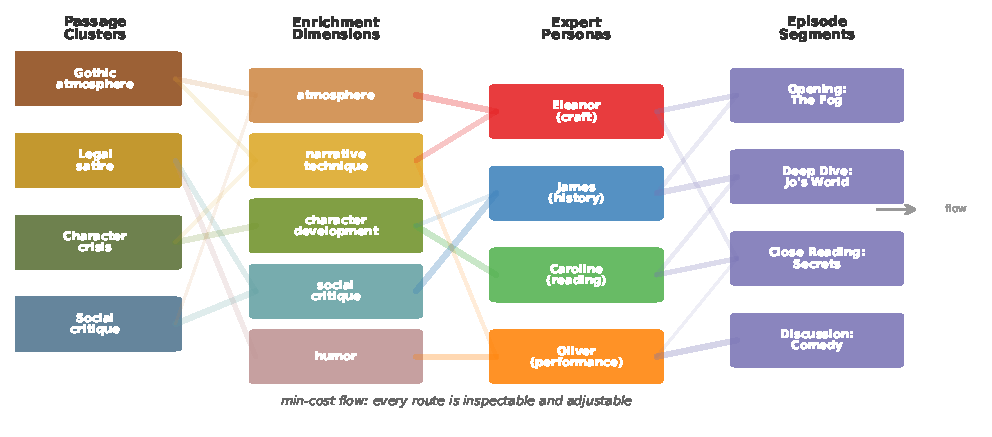
\includegraphics[width=0.85\linewidth]{sankey_flow.pdf}
\vspace{-1em}
\caption{\small Passages flow through enrichment dimensions and expert
  demand nodes to episode segments.  Every arc is inspectable and adjustable.}
\label{fig:flow}
\vspace{-0.8em}
\end{figure}

The expert personas are, deliberately, \emph{stereotypes}: the Marxist
always finds class struggle; the performer always finds comedy; the
close reader always finds prose rhythm. The generated discussions are
closer to parody than scholarship---each configuration produces a
recognisably different \emph{caricature} of academic discourse.  This
is the point.  By making the stereotypes explicit and
adjustable---encoded as demand vectors rather than implicit in a
prompt---the system turns editorial bias into a first-class object
that can be inspected, compared, and argued about.
Every editorial decision is inspectable and manipulable.
Twenty
configurations, varying panel composition and arc emphasis, produce
measurably different outputs: different passage selections (mean
pairwise Jaccard similarity~0.52), different vocabulary, and different
grammatical registers, confirmed by corpus comparison methods
\citep{kilgarriff2001comparing}.  What happens when we remove the
social historian?  Double a character arc?  Replace the close reader
with a comedian?  The answers are computable, and the differences are
legible.

We do not claim the generated podcasts are good---they are fluent,
structured, and plausible-sounding, which is precisely the problem
with LLM-generated academic discussion \citep{doshi2024generative}.
Following Boden's \citeyearpar{boden2004creative} taxonomy, the system
performs combinational creativity, but the \emph{interesting}
creativity is the user's: exploring the configuration space and
confronting the stereotypes that make the machinery work.
The system's value is diagnostic, turning a black-box pipeline into a
navigable space of configurations.
It is no accident that \textit{Bleak House} centres on the law:
lawyers reviewing documents under constraints need inspectable,
manipulable thinking tools at least as much as literary critics do.

\vspace{0.2em}
\noindent\textbf{Keywords:} optimal transport, min-cost flow, RAG, LLM stereotypes, editorial decision spaces

\vspace{-0.3em}
\bibliographystyle{plainnat}
\bibliography{refs}

\end{document}
